\documentclass{article}

% packages
\usepackage{amsmath, amsthm, thmtools, amsfonts, amssymb, luacode, catchfile, tikzducks, hyperref, ifthen}
\ifcsname c@kobocompile\endcsname
	\usepackage[a5paper, total={1072pt, 1448pt}, margin=10pt, includeheadfoot]{geometry} % set page margins
\else
	\usepackage[a4paper, margin=50pt, includeheadfoot]{geometry}
\fi
\usepackage[shortlabels]{enumitem}
\usepackage[skip=3pt, indent=0pt]{parskip}

% language
\usepackage[bidi=basic, layout=tabular, provide=*]{babel}
\ifcsname c@english\endcsname
	\babelprovide[main, import]{english}
\else
	\babelprovide[main, import]{hebrew}
	\babelprovide{rl}
\fi
%\babelfont{rm}{Libertinus Serif}
\babelfont{rm}[Renderer=Harfbuzz]{Libertinus Serif}
\babelfont{sf}{Libertinus Sans}
\babelfont{tt}{Libertinus Mono}

% style
\AddToHook{cmd/section/before}{\clearpage}	% Add line break before section
\linespread{1.3}
\setcounter{secnumdepth}{0}		% Remove default number tags from sections, this won't do well with theorems
\AtBeginDocument{\setlength{\belowdisplayskip}{3pt}}
\AtBeginDocument{\setlength{\abovedisplayskip}{3pt}}
\graphicspath{ {../images/} }

% operators
\DeclareMathOperator\cis{cis}
\DeclareMathOperator\Sp{Sp}
\DeclareMathOperator\tr{tr}
\DeclareMathOperator\im{Im}
\DeclareMathOperator\re{Re}
\DeclareMathOperator\diag{diag}
\DeclareMathOperator*\lowlim{\underline{lim}}
\DeclareMathOperator*\uplim{\overline{lim}}
\DeclareMathOperator\rng{rng}
\DeclareMathOperator\Sym{Sym}
\DeclareMathOperator\Arg{Arg}
\DeclareMathOperator\Log{Log}
\DeclareMathOperator\dom{dom}
\DeclareMathOperator\supp{Supp}
\DeclareMathOperator\var{Var}
\DeclareMathOperator\cov{Cov}

% commands
%\renewcommand\qedsymbol{\textbf{מש''ל}}
%\renewcommand\qedsymbol{\fbox{\emoji{lizard}}}
\newcommand{\Aa}[0]{\mathcal{A}}
\newcommand{\Bb}[0]{\mathcal{B}}
\newcommand{\CC}[0]{\mathbb{C}}
\newcommand{\Cc}[0]{\mathcal{C}}
\newcommand{\EE}[0]{\mathbb{E}}
\newcommand{\FF}[0]{\mathbb{F}}
\newcommand{\Ff}[0]{\mathcal{F}}
\newcommand{\Ii}[0]{\mathcal{I}}
\newcommand{\Gg}[0]{\mathcal{G}}
\newcommand{\Ll}[0]{\mathcal{L}}
\newcommand{\Mm}[0]{\mathcal{M}}
\newcommand{\NN}[0]{\mathbb{N}}
\newcommand{\Nn}[0]{\mathcal{N}}
\newcommand{\PP}[0]{\mathbb{P}}
\newcommand{\Pp}[0]{\mathcal{P}}
\newcommand{\QQ}[0]{\mathbb{Q}}
\newcommand{\RR}[0]{\mathbb{R}}
\newcommand{\Rr}[0]{\mathcal{R}}
\newcommand{\Ss}[0]{\mathcal{S}}
\newcommand{\TT}[0]{\mathbb{T}}
\newcommand{\Uu}[0]{\mathcal{U}}
\newcommand{\Vv}[0]{\mathcal{V}}
\newcommand{\Ww}[0]{\mathcal{W}}
\newcommand{\ZZ}[0]{\mathbb{Z}}
\newcommand{\acts}[0]{\circlearrowright}
\newcommand{\explain}[2] {
	\begin{flalign*}
		 && \text{#2} && \text{#1}
	\end{flalign*}
}
\newcommand{\maketitleprint}[0]{ \begin{center}
	%\begin{tikzpicture}[scale=3]
	%	\duck[graduate=gray!20!black, tassel=red!70!black]
	%\end{tikzpicture}	
	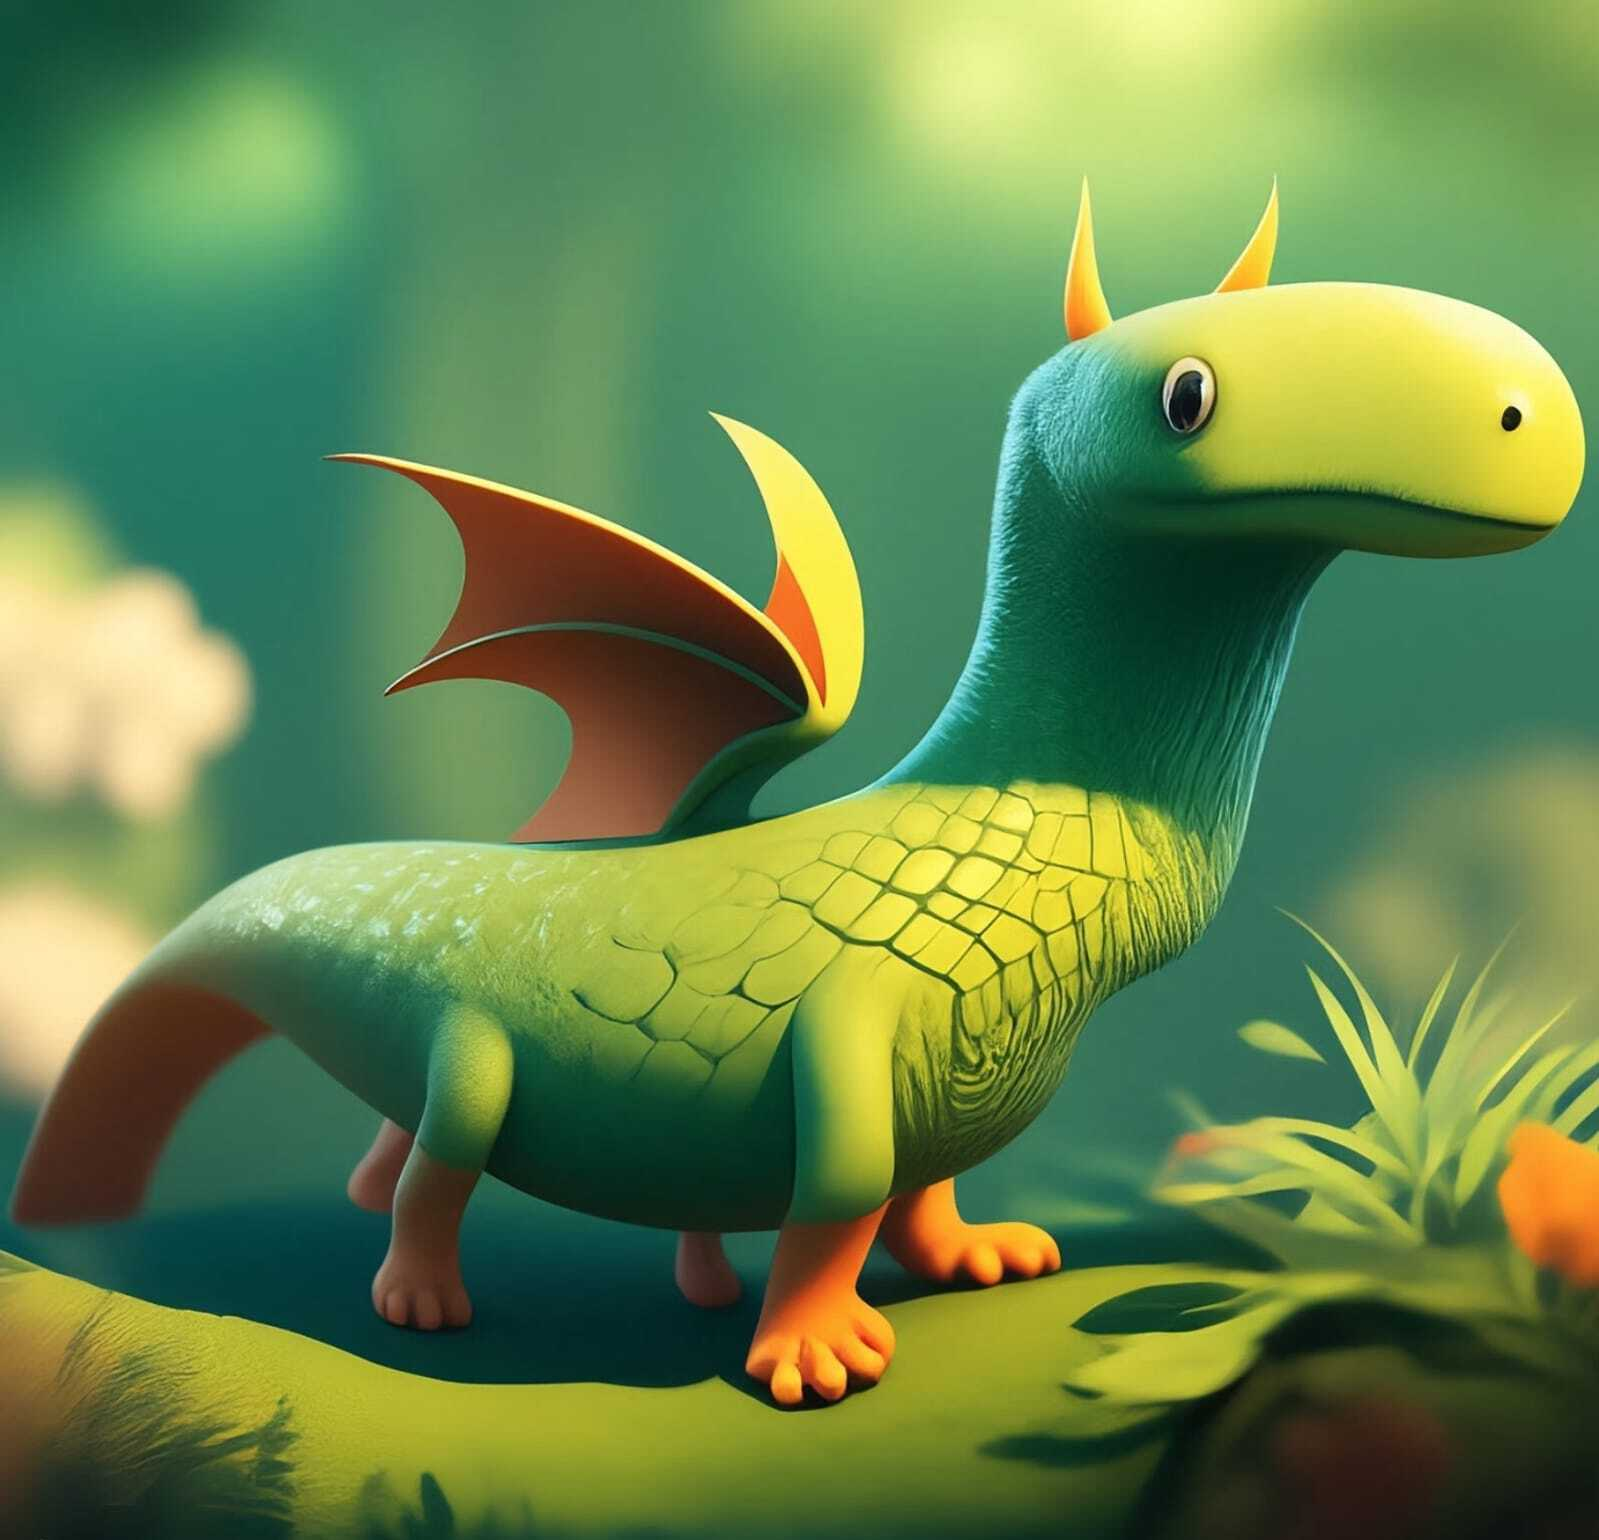
\includegraphics[width=6cm]{cover}
\end{center}
}

% theorem commands
\newtheoremstyle{c_remark}
	{}	% Space above
	{}	% Space below
	{}% Body font
	{}	% Indent amount
	{\bfseries}	% Theorem head font
	{}	% Punctuation after theorem head
	{.5em}	% Space after theorem head
	{\thmname{#1}\thmnumber{ #2}\thmnote{ \normalfont{\text{(#3)}}}}	% head content
\newtheoremstyle{c_definition}
	{3pt}	% Space above
	{3pt}	% Space below
	{}% Body font
	{}	% Indent amount
	{\bfseries}	% Theorem head font
	{}	% Punctuation after theorem head
	{.5em}	% Space after theorem head
	{\thmname{#1}\thmnumber{ #2}\thmnote{ \normalfont{\text{(#3)}}}}	% head content
\newtheoremstyle{c_plain}
	{3pt}	% Space above
	{3pt}	% Space below
	{\itshape}% Body font
	{}	% Indent amount
	{\bfseries}	% Theorem head font
	{}	% Punctuation after theorem head
	{.5em}	% Space after theorem head
	{\thmname{#1}\thmnumber{ #2}\thmnote{ \text{(#3)}}}	% head content

\ifcsname c@english\endcsname
	\theoremstyle{plain}
	\newtheorem{theorem}{Theorem}[section]
	\newtheorem{lemma}[theorem]{Lemma}
	\newtheorem{proposition}[theorem]{Proposition}
	\newtheorem*{proposition*}{Proposition}
	%\newtheorem{corollary}[theorem]{אין חלופה עברית}

	\theoremstyle{definition}
	\newtheorem{definition}[theorem]{Definition}
	\newtheorem*{definition*}{Definition}
	\newtheorem{example}{Example}[section]
	\newtheorem{exercise}{Exercise}[section]

	\theoremstyle{remark}
	\newtheorem*{remark}{Remark}
	\newtheorem*{solution}{Solution}
	\newtheorem{conclusion}[theorem]{Conclusion}
	\newtheorem{notation}[theorem]{Notation}
\else
	\theoremstyle{c_plain}
	\newtheorem{theorem}{משפט}[section]
	\newtheorem{lemma}[theorem]{למה}
	\newtheorem{proposition}[theorem]{טענה}
	\newtheorem*{proposition*}{טענה}
	%\newtheorem{corollary}[theorem]{אין חלופה עברית}

	\theoremstyle{c_definition}
	\newtheorem{definition}[theorem]{הגדרה}
	\newtheorem*{definition*}{הגדרה}
	\newtheorem{example}{דוגמה}[section]
	\newtheorem{exercise}{תרגיל}[section]

	\theoremstyle{c_remark}
	\newtheorem*{remark}{הערה}
	\newtheorem*{solution}{פתרון}
	\newtheorem{conclusion}[theorem]{מסקנה}
	\newtheorem{notation}[theorem]{סימון}
\fi

% Questions related commands
\newcounter{question}
\setcounter{question}{1}
\newcounter{sub_question}
\setcounter{sub_question}{1}

\ifcsname c@english\endcsname
	\newcommand{\question}[1][0]{
		\ifthenelse{#1 = 0}{}{\setcounter{question}{#1}}
		\section{Question \arabic{question}}
		\addtocounter{question}{1}
		\setcounter{sub_question}{1}
	}

	\newcommand{\subquestion}[1][0]{
		\ifthenelse{#1 = 0}{}{\setcounter{sub_question}{#1}}
		\subsection{Part \alph{sub_question}}
		\addtocounter{sub_question}{1}
	}
\else
	\newcommand{\question}[1][0]{
		\ifthenelse{#1 = 0}{}{\setcounter{question}{#1}}
		\section{שאלה \arabic{question}}
		\addtocounter{question}{1}
		\setcounter{sub_question}{1}
	}

	\newcommand{\subquestion}[1][0]{
		\ifthenelse{#1 = 0}{}{\setcounter{sub_question}{#1}}
		\subsection{סעיף \localecounter{letters.gershayim}{sub_question}}
		\addtocounter{sub_question}{1}
	}
\fi

% import lua and start of document
\directlua{common = require ('../common')}

\GetEnv{AUTHOR}

% headers
\author{\AUTHOR}
\date\today

\title{פתרון מטלה 02 --- מבנים אלגבריים 1 (80445)}

\begin{document}
\maketitle
\maketitleprint{}

\Question{}
נוכיח שכל חבורה ציקלית איזומורפית ל־$\ZZ$ או ל־$\ZZ/n$ בלבד.
\begin{proof}
	תהי חבורה $G$ ציקלית הנוצרת על־ידי $\langle a \rangle$, כאשר $a \in G$. \\*
	נניח תחילה כי $G$ סופית, ולכן קיים $n > 0$ כך ש־$a^n = e$ כאשר $e$ איבר נייטרלי של $G$. \\*
	נסיק אם כן כי הסדר של $G$ הוא בעצמו $n$, ונגדיר פונקציה $\varphi : \ZZ \to G/n$ על־ידי
	\[
		\varphi(n) = a^n
	\]
	נשים לב שלכל $x, y \in \ZZ/n$ מתקיים $\varphi(x +_n y) = a^{x + y} = a^x a^y = \varphi(x) \varphi(y)$ ולכן על־פי התנאי ההכרחי $\varphi$ הומומורפיזם. \\*
	מהגדרת החבורה וההומומורפיזם ניתן להסיק בנקל כי היא חד־חד ערכית, ומהגדרתה הישירה נסיק כי היא גם על, ולכן היא איזומורפיזם, ובהתאם $G \xrightarrow{\sim} \ZZ/n$. \\*
	נניח עתה כי $G$ איננה סופית ונגדיר את $\varphi : G \to \ZZ$ באותו האופן אשר הוגדרה בו עד כה, אך נגדיר גם $\varphi(-n) = {(a^{-1})}^n$. \\*
	הפונקציה $\varphi$ מוגדרת לכל $n \in \ZZ$, ומהציקליות אנו יודעים שכל איבר $x \in G$ ניתן לכתיבה כ־$a^n$ שלם כלשהו, ולכן נסיק כי $\varphi$ היא איזומורפיזם ובהתאם $G \xrightarrow{\sim} \ZZ$. \\*
	מצאנו כי $G$ ציקלית איזומורפית ל־$\ZZ/n$ כלשהו או ל־$\ZZ$.
\end{proof}

\Question{}
\Subquestion{}
נוכיח שלכל $n \ge 1$ החבורה $S_n$ נוצרת על־ידי $H = \langle (i j) \mid 1 \le i < j \le n \rangle$.
\begin{proof}
	יהי $l$־מחזור $\sigma = (\lambda_1 \hdots \lambda_l)$ ויהי $\tau = (\lambda_l \lambda_{l + 1})$, אז $\tau \circ \sigma = (\lambda_1 \hdots \lambda_l \lambda_{l + 1})$ $l + 1$־מחזור. \\*
	זאת אנו מקבלים על־ידי בדיקה ישירה של הפונקציה. נוכל להשתמש בטענה כדי להוכיח שכל $l$־מחזור נתון ניתן להרכבה על־ידי $l$ $2$־מחזורים. \\*
	על־ידי צירוף הטענה שכל תמורה ניתנת לייצוג על־ידי הרכבת מספר סופי של מחזורים נקבל כי $H = S_n$.
\end{proof}

\Subquestion{}
נוכיח כי גם $H_1 = \langle (i, i + i) \mid 1 \le i < n \rangle$ יוצרת את $S_n$.
\begin{proof}
	נבחין כי הרכבת המחזורים $(a t)(t b)(ta)$ מניבה את המחזור $(a b)$, ונוכיח באינדוקציה שכל המחזורים מהצורה $(1, n)$ מוכלים ב־$H_1$. \\*
	\textbf{בסיס אינדוקציה:} נראה כי $(1 2)(2 3)(2 1) = (1 3)$. \\*
	\textbf{מהלך אינדוקציה:} נניח כי $(1 n) \in H_1$ ולכן $(1 2)(n+1\ 2)(2 1) = (1\ n + 1)$, וקיבלנו כי הטענה מתקיימת. \\*
	עתה נראה כי לכל $1 \le x, y \le n$ מתקיים $(1 x), (1 y) \in H_1$ ולכן ההרכבה $(x 1)(1 y)(x 1) = (x y) \in H_1$ וקיבלנו כי תנאי הסעיף הקודם מתקיימים ונובע $H_1 = H = S_n$.
\end{proof}

\Subquestion{}
נוכיח כי גם $H_2 = \langle (1\ 2)(1\ 2 \hdots n) \rangle$ יוצר את $S_n$.
\begin{proof}
	נראה כי
	\[
		{(1\ 2 \hdots n)}^k
		(1\ 2)
		= (k\ k+1)
	\]
	נובע ישירות מתהליך ההרכבה, לכן $H_2 = H_1$ ובהתאם גם $H_2 = S_n$.
\end{proof}

\Question{}
יהי $n \ge 3$ ונגדיר $\sigma, \tau \in S_n$ על־ידי
\[
	\sigma(k) = k + 1 \mod n, \qquad \tau(k) = n - k + 1
\]
ונגדיר את החבורה הדיהדרלית $D_n = \langle\sigma, \tau\rangle \le S_n$.

\Subquestion{}
נשים לב שהחבורה $D_4$ זהה להגדרתה המקורית על־ידי ריבוע. אני משוכנע.

\Subquestion{}
נראה כי
\[
	\tau(\tau(k)) = n - (n - k + 1) + 1 = k \implies \tau^2 = Id
\]
בנוסף נבחין כי מהגדרתה נובע כי $\sigma^t(k) = k + t \mod n$ ולכן כאשר $t = n$ נקבל
\[
	\sigma^n(k) = k + n \mod n = k \implies \sigma^n = Id
\]
נבחין כי עבור הפעולות מודולו מתקיים
\[
	(\sigma^t \circ \tau)(k)
	= (n - k + 1) + t
	= n - k + 1 + t
	= n - (k - t) + 1
	= \tau \circ \sigma^{n - t}
\]
ולכן כל איבר ב־$D_n$ ניתן לכתיבה בצורה $\tau^{0, 1} \sigma^n$ ולכן בהתאם נקבל כי $|D_n| = 2n$.

\Subquestion{}
נבדוק לאילו $n \ge 3$ החבורה $D_n$ מכילה תת־חבורה איזומורפית $\ZZ/2 \times \ZZ/2$. \\*
נבחין כי כל תנאי ש־$n$ זוגי נוכל לבחור $\langle \tau, \sigma^{\frac{n}{2}} \rangle$ תת־חבורה בעלת ארבעה איברים ונוכל להגדיר $\varphi : D_4 \xrightarrow{\sim} \ZZ/2 \times \ZZ/2$ על־ידי $\varphi(\tau^x \sigma^y) = (x, y)$.

\Question{}
\Subquestion{}
נוכיח שמתקיים לכל $a, b \in \NN$
\[
	\text{lcm}(a, b) = \frac{ab}{\gcd(a, b)}
\]
ואף שערך זה קיים תמיד והוא יחיד.
\begin{proof}
	נגדיר $d = \gcd(a, b)$. נראה כי $d \mid b$ ולכן נגדיר $b_1 = b/d$. \\*
	בהתאם $\gcd(a, b_1) = 1$, כנביעה מהגדרת המחלק המשותף המקסימלי ישירות. \\*
	נגדיר גם $a_1 = a / d$ ולכן $a_1 b_1 d = ab$. \\*
	נשים לב שמהגדרת $d$ נובע כי אין מספר קטן יותר כך ש־$e b_1 = b$ או $e a_1 = a$ ובהתאם $a_1 b_1$ הוא הכפולה המינימלית המשותפת ומתקיים
	\[
		\text{lcm}(a, b) = \frac{ab}{\gcd(a, b)}
	\]
	והוא קיים לכל שני מספרים טבעיים ויחיד מיחידות $\gcd$.
\end{proof}

\Subquestion{}
נוכיח כי מתקיים גם
\[
	\text{lcm}(a, b)\ZZ = a\ZZ \cap b\ZZ
\]
\begin{proof}
	נשים לב כי קבוצת המספרים המתחלקים על־ידי $a$ ו־$b$ על־פי הגדרה מתחלקת גם ב־$\text{lcm}(a, b)$, ולכן
	\[
		\text{lcm}(a, b)\ZZ \subseteq a\ZZ \cap b\ZZ
	\]
	נראה גם כי כל מספר $c \in \text{lcm}(a, b)\ZZ$ הוא כפולה של $a$ וכן של $b$ מהגדרת הכפולה המינימלית המשותפת, ולכן נובע
	\[
		\text{lcm}(a, b)\ZZ = a\ZZ \cap b\ZZ
	\]
\end{proof}

\Question{}
\Subquestion{}
תהינה $H \le G$ חבורה ותת־חבורה שלה. נוכיח שיש פונקציה הפיכה בין $G / H$ לבין $H \backslash G$.
\begin{proof}
	יהי $a, b \in G$, אם $a H = b H$ אם ורק אם קיימים איברים $h_1, h_2 \in H$ כך ש־$a h_1 = b h_2$ ולכן גם $h_1^{-1} a^{-1} = h_2^{-1} b^{-1}$. \\*
	אבל $h_1^{-1}, h_2^{-1} \in H$ שכן היא סגורה להופכי ונקבל כי $H a^{-1} = H b^{-1}$ אם ורק אם $a H = b H$. \\*
	נגדיר פונקציה $\varphi : G/H \to H\backslash G$ על־ידי
	\[
		\varphi(a H) = H a^{-1}
	\]
	הפונקציה היא חד־חד ערכית על־פי הטענה שהוכחנו זה עתה, ונראה כי היא על: \\*
	נבחר $H a$ מחלקה ימנית כלשהי ב־$H \backslash G$. אז $\varphi(a^{-1} H) = H a$ לכל $a \in G$ ולכן היא על. \\*
	מצאנו כי $G / H \xrightarrow{\sim} H \backslash G$. \\*
	נסיק כי החבורות מאותו סדר, ולכן $|G : H|$ הוא בלתי תלוי בבחירת מחלקה ימנית או שמאלית.
\end{proof}

\Subquestion{}
תהינה $K \le H \le G$ חבורה ותת־חבורות כך ש־$G / H$ ו־$H / K$ סופיות. \\*
נוכיח כי $G / K$ סופי ומתקיים $|G/K| = |G/H| \cdot |H/K|$.
\begin{proof}
	יהי $g \in G, h \in H$ ונראה כי $gH, hK$ הן מחלקות של $G/H$ ו־$H/K$ בהתאמה. \\*
	לכל $h \in H$ קיים $g_1 \in G$ כך ש־$g = g_1 h$.
	לכן $g K = g_1 h K = g_1 (h K)$. \\*
	נשים לב שיש כמות סופית של מחלקות $h K$ ו־$g_1 H$ ולכן יש כמות קומבינציות סופית של בחירות כאלה שנוכל לעשות (לבחירות זרות). \\*
	מכאן נסיק ש־$G / K$ עצמה היא סופית. \\*
	בחירת $g, h$ היא קומבינציה בלתי תלויה ולכן חל עליה חוק הכפל של קומבינטוריקה ומתקיים $|G/K| = |G/H| \cdot |H/K|$.
\end{proof}

\Subquestion{}
נמצא את האינדקס $|SL_n(\FF_p) : GL_n(\FF_p)|$ \\*
נגדיר $H = SL_n(\FF_p)$, אז $\forall h \in H : |h| = 1$ על־פי הגדרת תת־החבורה. \\*
תהי $a \in GL_n(\FF_p)$, ונגדיר $k = |a|$, ידוע כי $0 < k < p$ בהתאם להגדרת השדה. \\*
מתקיים גם $\forall h \in H : |ah| = |a| \cdot |h| = k$ על־פי חוקי דטרמיננטות. \\*
נסיק כי כל מחלקת שקילות שומרת על גודל הדטרמיננטה, וידוע כי ישנם $k - 1$ גדלים אפשריים, ולכן נסיק גם
\[
	|SL_n(\FF_p) : GL_n(\FF_p)| = k - 1
\]

\Question{}
נוכיח שניתן ליצור את $SL_n(\ZZ)$ על־ידי $n^2 - n$ איברים.
\begin{proof}
	נבחן את המטריצות ההפיכות בעלות דטרמיננטה $1$ מעל השלמים. \\*
	כל מטריצה הפיכה ניתן ליצור מצירוף של מטריצות אלמנטריות, ולכן נבחן את הקבוצה שלהן בלבד. \\*
	לא יתכן ששורה תהיה מוכפלת בסקלר שכן על שורה אחרת להיות מוכפלת בסקלר ההופכי, והוא לא קיים בשלמים, לכן כל איברי המטריצה הם $0$ או $1$. \\*
	בהתאם יש רק שני סוגים של פעולות אלמנטריות על המטריצה, החפלת שורות וצירוף לינראי של שורות. \\*
	על־ידי השיטה $\forall a, b \in \ZZ: a := a + b, b := a - b, a := a - b$ ניתן להחליף את ערכם של שני משתנים, נשתמש באלגוריתם זה כדי להיות מסוגלים להחליף ערכי שורות שלמות על־ידי הוספת צירופים לינאריים של שורות.
	מסיבה זו אין צורך לכלול את המטריצות האלמנטריות להחלפת שורות בקבוצה, ונשארו מטריצות הוספת הצירוף הלינארי. \\*
	נשים לב שנוכל להוסיף כל שורה לכל שורה שונה ממנה שוב ושוב כדי להגיע לצירוף הלינארי השלם הרצוי, ולכן ישנן $n(n - 1)$ מטריצות כאלה. \\*
	נוכל כמובן להשתמש בפעולות ההופכיות שלהן הנוצאות על־ידיהן בבנייה כדי להגיע לחיסור שורות, ולכן קבוצת מטריצות זו בונה את $SL_n(\ZZ)$.
\end{proof}

\end{document}
